\documentclass{article}
\usepackage{graphicx}
\usepackage{hyperref}
\usepackage{color}
\usepackage{wasysym}

\begin{document}

\title{Poppy Humanoid Robot Mounting Guide}
\author{Manon Cortial, Generation Robots}

\maketitle

\section{Introduction}

\subsection{The Poppy project}

Poppy is an open hardware and open-source robotics project. It has been designed to allow researchers and students to easily remove and replace some parts of the body. 

For example,   different leg shapes have been tested on the Poppy Humanoid robot to make the robot walk.

 \begin{center}
  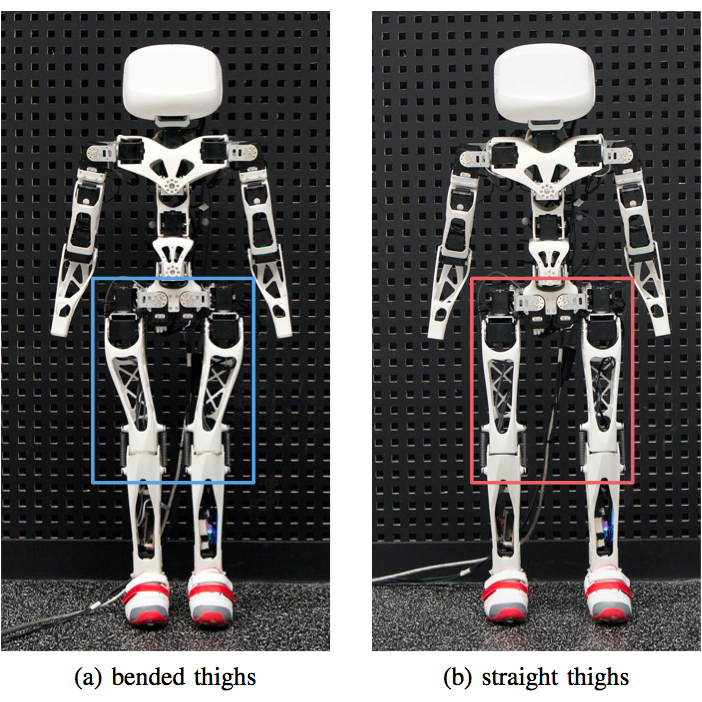
\includegraphics[width=0.6\textwidth]{humanoids2013_Experiments}
 \end{center}


\subsection{\textcolor{red}{Safety warning}}

The Poppy humanoid robot is built using mainly MX-28 Dynamixel servomotors, which are pretty powerful and may be harmful to your fingers or materials.

So be very careful and put the robot in a free space while testing your programs.

\section{Dynamixel hardware}

The Poppy Humanoid robot is mainly built with \href{http://www.generationrobots.com/en/401858-servomotor-dynamixel-mx-28at.html}{MX-28AT Dynamixel servomotors} (MX-28T are the previous version and can be used without any problem). The other servomotors are MX-64T (bigger and stronger) and AX-12A (smaller, used for the head).

Each Dynamixel servomotor embeds an electronical board allowing it to receive different kind of orders (about goal, torque...) and communicate with other Dynamixel servos. Therefore, you can chain up several Dynamixel servomotors (each with a different ID) and command them all from one end of the chain: each servomotor will pass the orders to the next one. 

 \begin{center}
  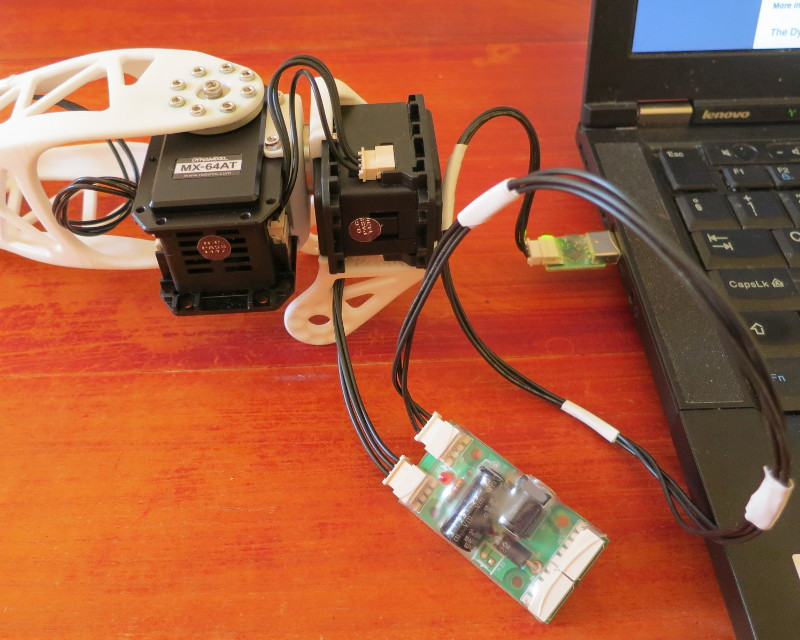
\includegraphics[width=0.6\textwidth]{daisy_link}
 \end{center}
 

\subsection{Putting the Dynamixel horns to zero}
\label{dynamixel-zero}

\textcolor{red}{\textbf{This step is critical to avoid damaging your Dynamixel servomotors !}}

When you receive your Dynamixel servomotors, the horns are not mounted. They are included in the packaging if the servo is packaged alone or packaged separately for 6-pieces bulks (see next section to know what horn goes to what servo).

When putting the controlled horn, be very careful to \textbf{put the dot on the horn at the same point than the dot on the servo axis}. Once the horn is put, it is most of the time \textbf{impossible to remove} ! This will ensure that the zero position of the servo matches with the zero position of the structure around.

 \begin{center}
  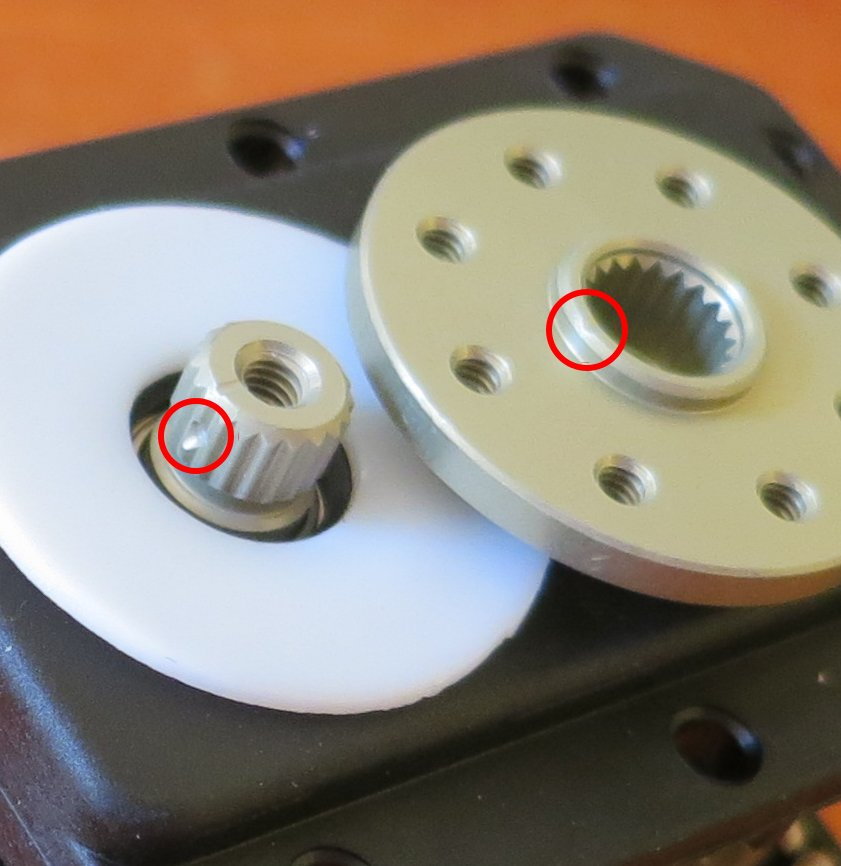
\includegraphics[height=0.55\textwidth]{zero}
  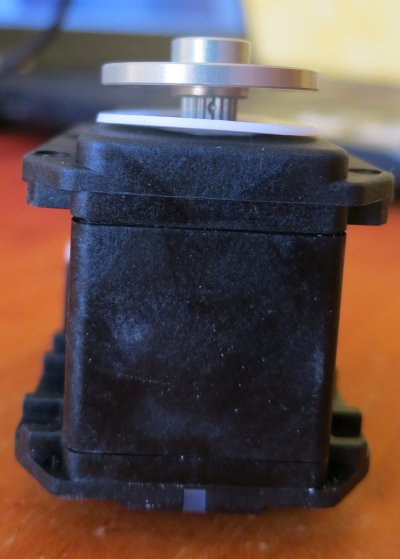
\includegraphics[height=0.55\textwidth]{zero2}
 \end{center}

On the outside of the horn, you also have three dots indicating the orientation. You should find the same three dots on structural parts, so be sure to match them.

 \begin{center}
  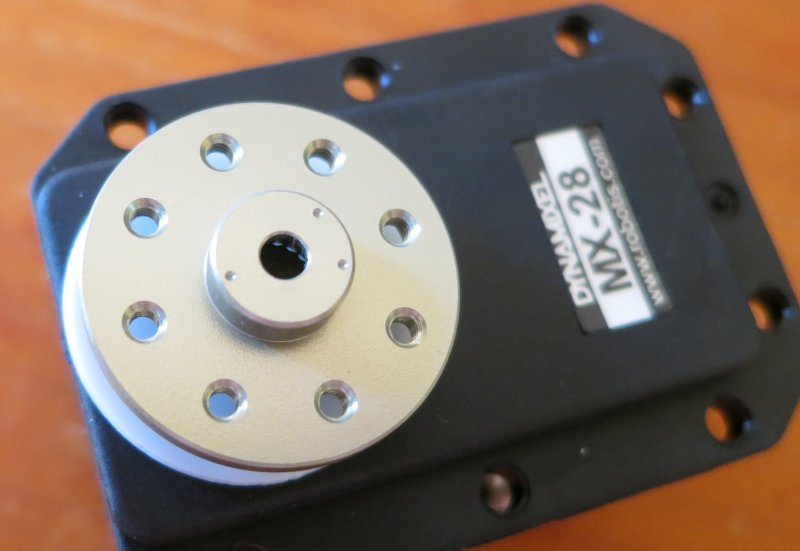
\includegraphics[width=0.6\textwidth]{zero3}
 \end{center}
\subsection{Horns of MX-28 and MX-64}

On each Dynamixel servotor apart from the AX-12A, you will have to mount a horn to the motor axis. Most of the time, you will also have to mout a free horn on the opposite side to provide better fixation points for the structure parts.

To mount the main horn, put the plastic ring (white or black) and drive the horn on the axis. \textbf{Be careful of the zero when putting the main horn!} Then put thread locker on the big screw and screw it in the middle.


 \begin{center}
  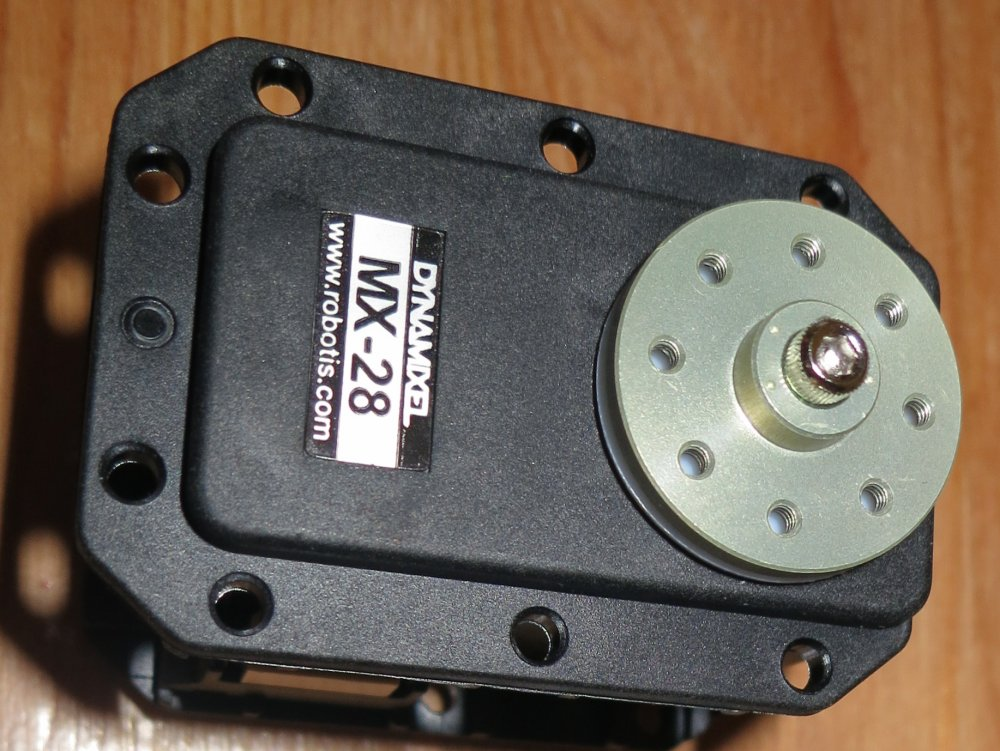
\includegraphics[width=0.5\textwidth]{MX28N}

Main horn mounted on a MX-28
 \end{center} 
 
 For the free horn, first clip the ball bearing and the cap on the side without shaft shoulder. Then put the horn on servomotor (with shaft shoulder on servo side). Put thread locker on the big screw and screw it. The horn should turn freely.

 
  \begin{center}
  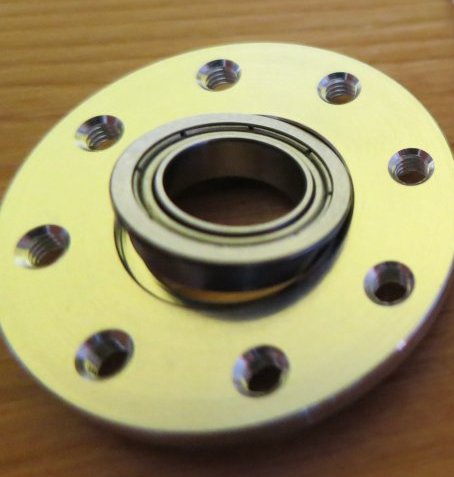
\includegraphics[height=0.3\textwidth]{MX64I1}
  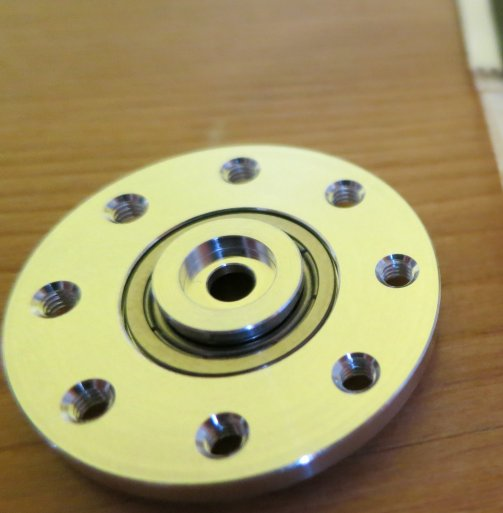
\includegraphics[height=0.3\textwidth]{MX64I2}
  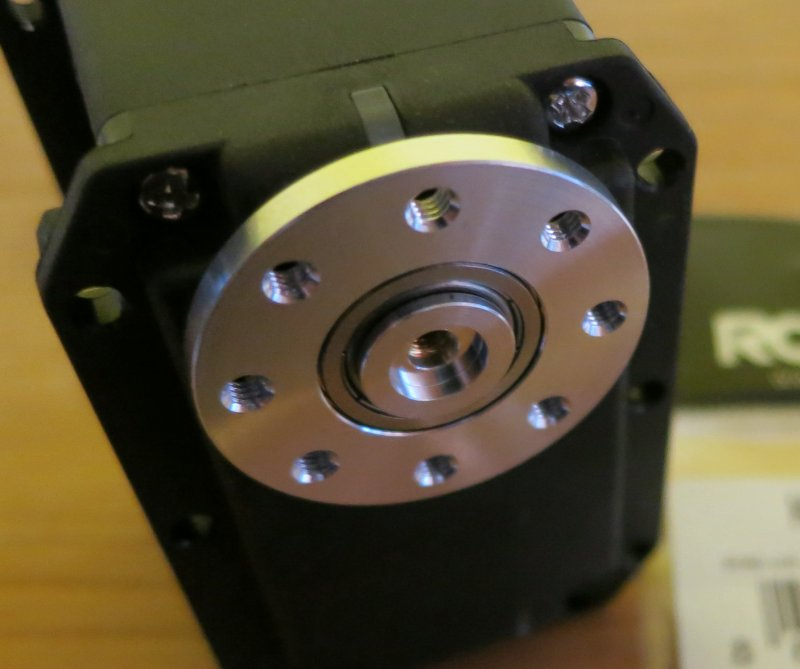
\includegraphics[height=0.3\textwidth]{MX64I3}

Free horn mounted on a MX-64
 \end{center}
 
Quick reminder of horn names and screw sizes:

\hspace{-6mm}\begin{tabular}{|c|c|c|c|c|c|}
\hline 
Servomotor & main horn & free horn & big horn screw & horn screws & case screws \\ 
\hline 
AX12-A & none & none & none & \diameter 2 & \diameter 2\\ 
\hline 
MX28 & HN07-N101 & HN07-I101 & \diameter 2.5x8mm & \diameter 2x3mm & \diameter 2.5x6mm  \\ 
\hline 
MX64 & HN05-N102 & HN05-I101 & \diameter 3x8mm & \diameter 2.5x4mm & \diameter 2.5x6mm  \\ 
\hline 
\end{tabular} 

You need  1.5mm for \diameter 2 screws, an allen wrench of size 2mm for \diameter 2.5 screws and 2.5mm for \diameter 3 screws.

\subsection{Putting the nuts}

To attach structural parts on the body of the servomotors, you have to first insert the nuts in their sites. This step may be quite painful if you don't have elfic fingers.

Here's my tip: take the nut using thin tweezers and bring it in the site with the right orientation. Put the end of the tweezers in the hole to ensure good alignment. Then use flat pincers to ajust the nut.

 \begin{center}
  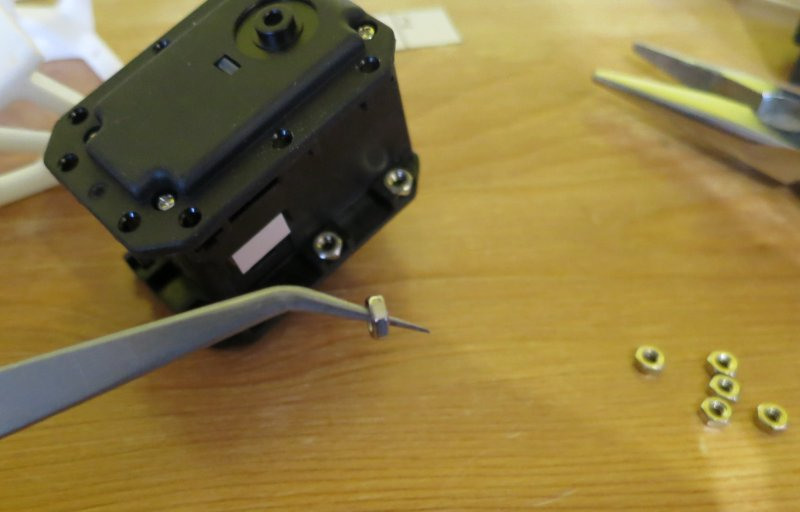
\includegraphics[width=0.55\textwidth]{nuts1}
  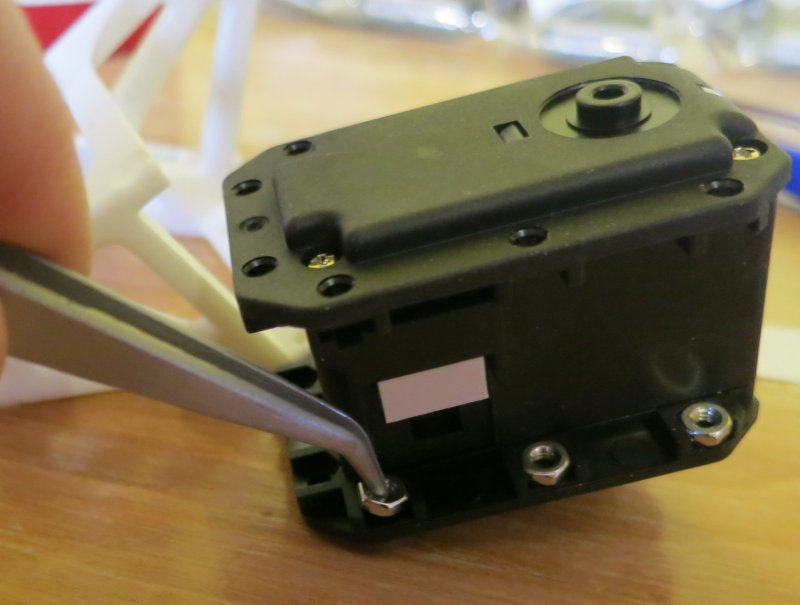
\includegraphics[width=0.55\textwidth]{nuts2}
  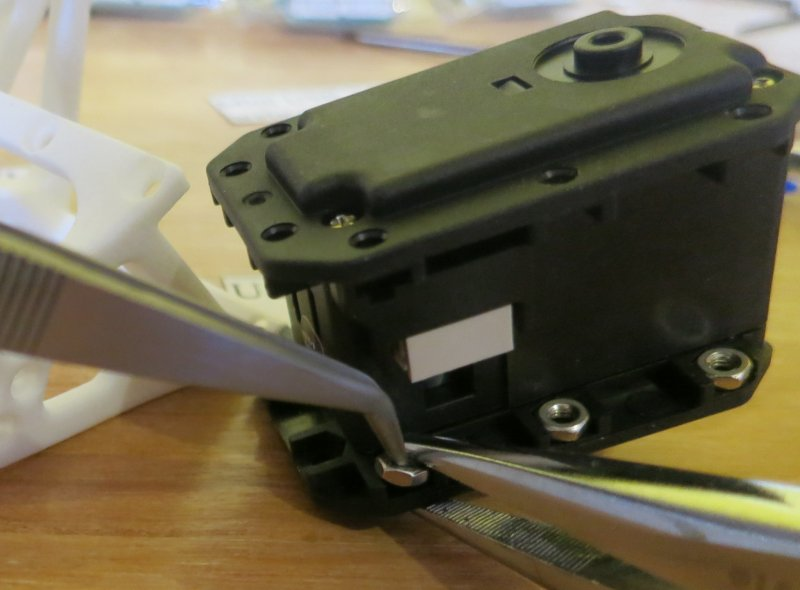
\includegraphics[width=0.55\textwidth]{nuts3}
 \end{center}
 
 These nuts correspond to diameter 2.5mm screws, allen wrench 2mm.
 
 To build a full Poppy Humanoid robot, an electrical screwdriver is strongly advised!

\section{Structural parts}

 \begin{center}
  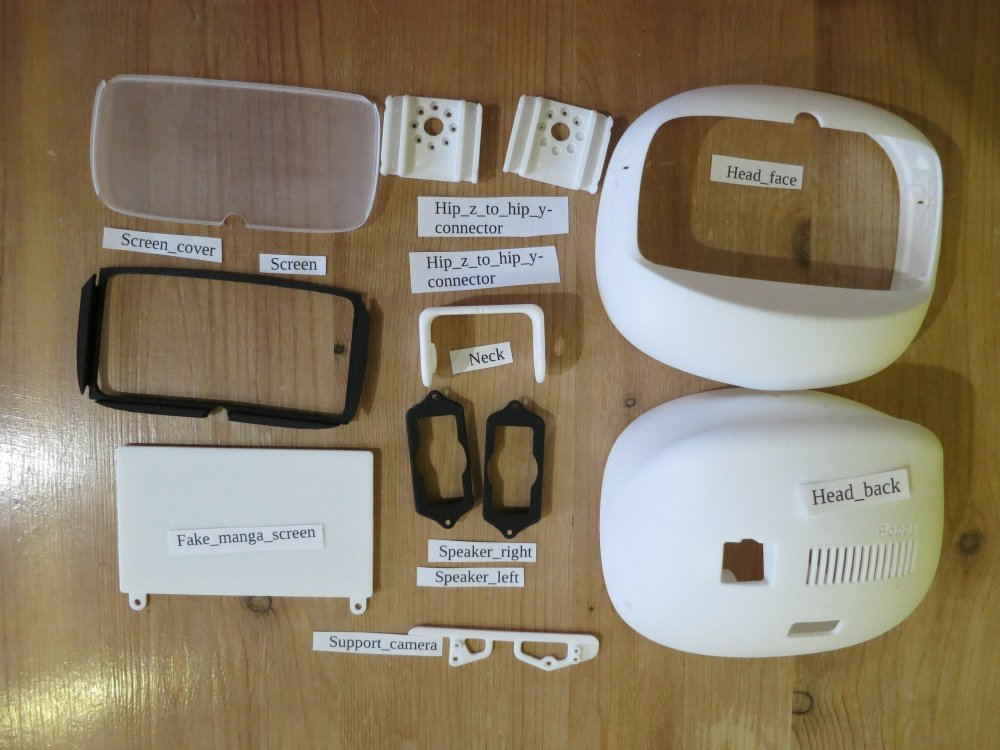
\includegraphics[width=0.9\textwidth]{parts_head}\\
  \vspace{1mm}
  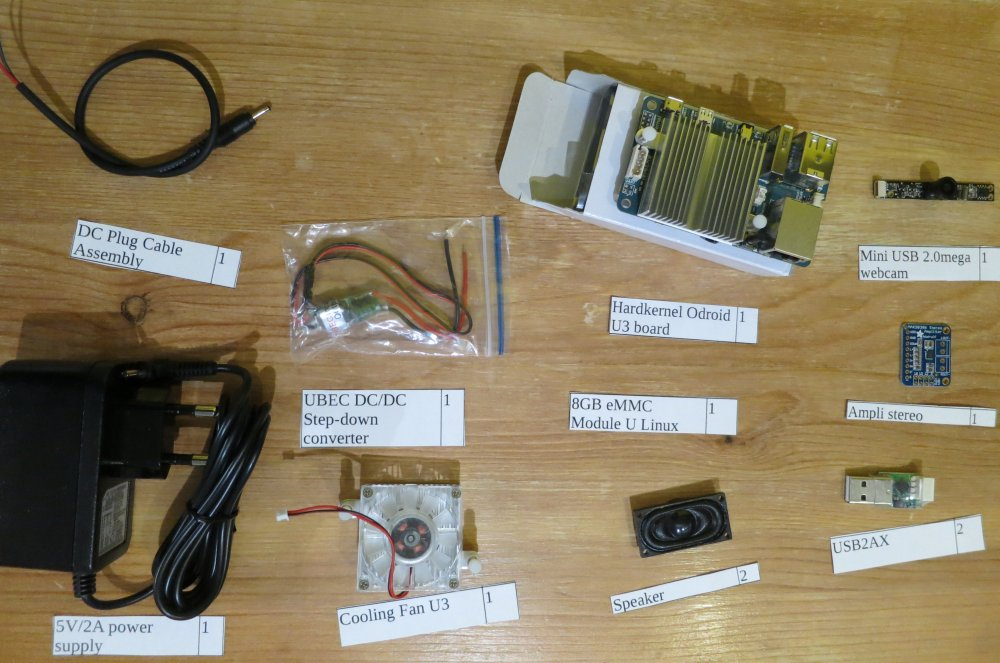
\includegraphics[width=0.9\textwidth]{parts_electronics}\\
  \vspace{1mm}
  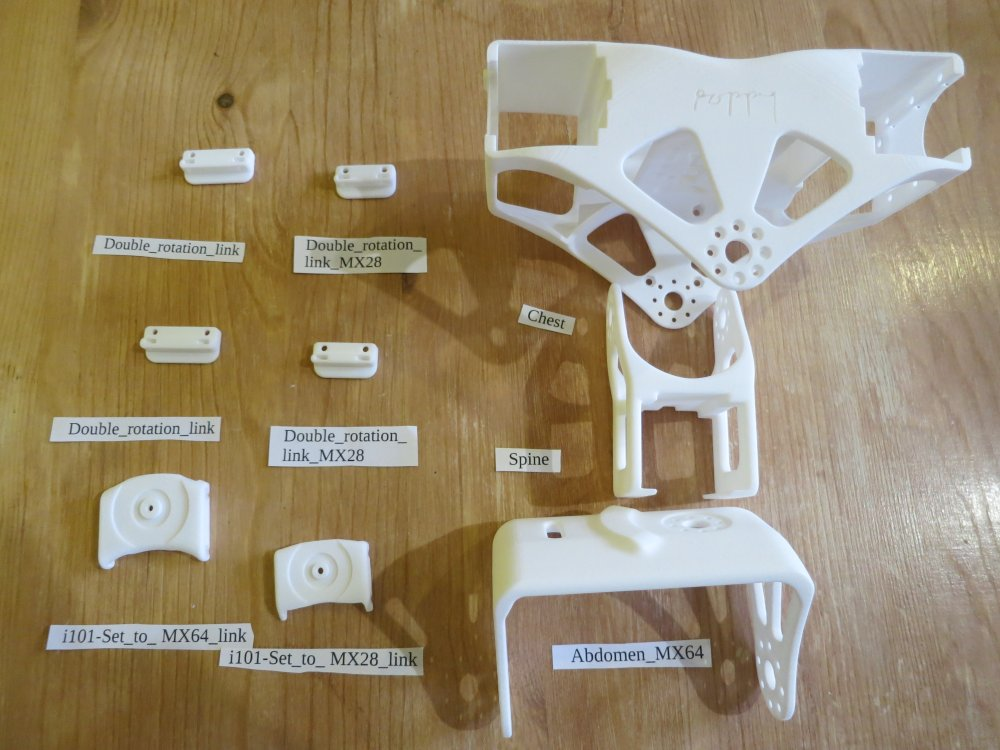
\includegraphics[width=0.9\textwidth]{parts_chest}\\
  \vspace{1mm}
  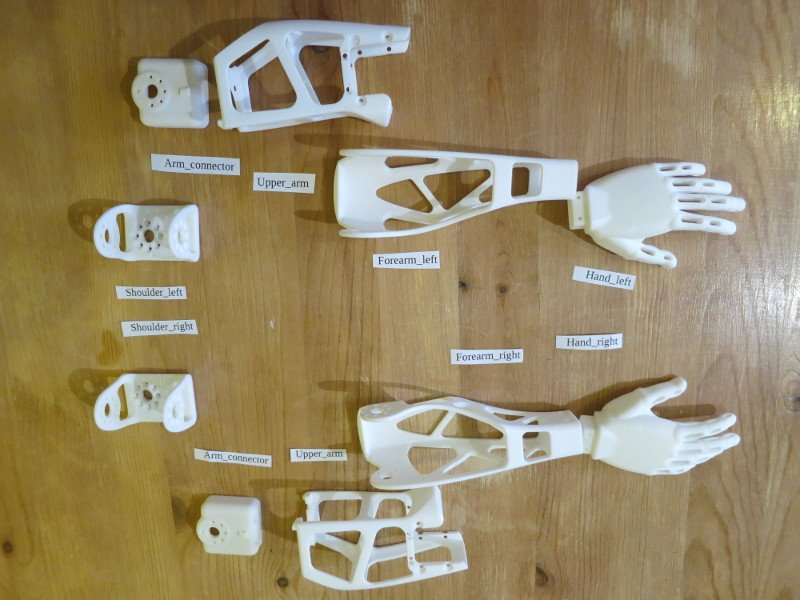
\includegraphics[width=0.9\textwidth]{parts_arms}\\
  \vspace{1mm}
  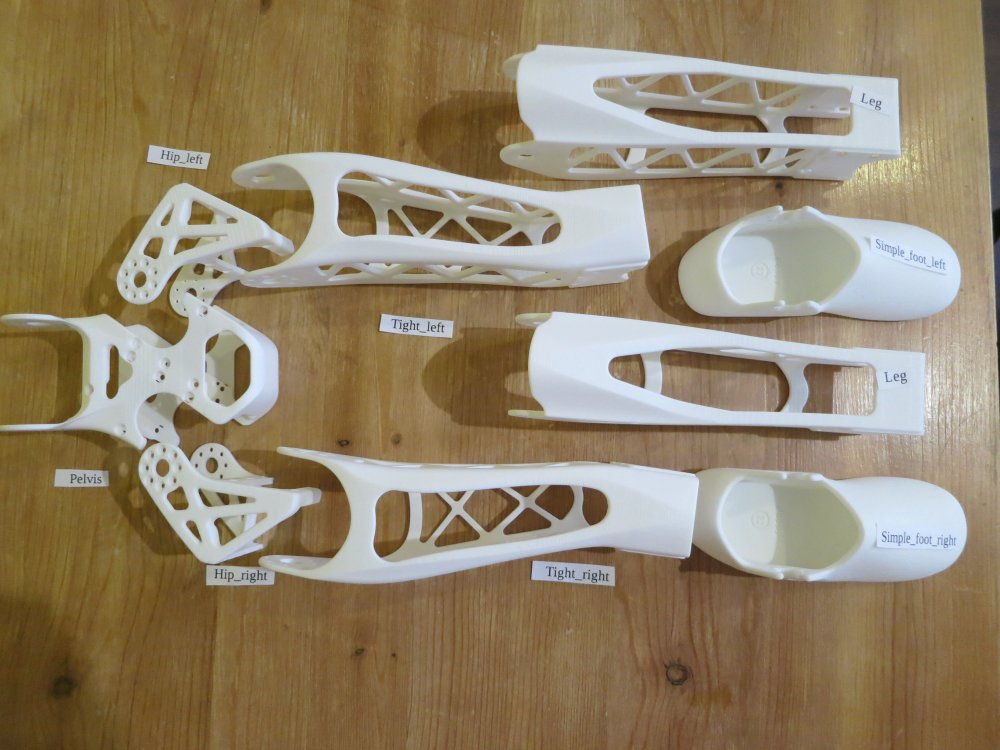
\includegraphics[width=0.9\textwidth]{parts_legs}
 \end{center}



\section{Assembly tips}

\subsection{Trunk} 
 
Documentation links:

\begin{itemize}
\item \textbf{\href{https://github.com/poppy-project/Robotis-library/blob/master/doc/en/double\_MX64\_assembly.md}{Double MX64}}
\item \textbf{\href{https://github.com/poppy-project/Robotis-library/blob/master/doc/en/double\_MX28\_assembly.md}{Double MX28}} Don't screw the i101-Set\_to\_ MX28\_link (the plastic part with a free horn on it) too tightly, or don't screw it at all since you will need to unscrew it during the trunk assembly.
\item \textbf{\href{https://github.com/poppy-project/Poppy-multiarticulated-torso/blob/master/doc/en/subassembly/spine\_assembly\_instructions.md}{Spine}}
\item \textbf{\href{https://github.com/poppy-project/Poppy-multiarticulated-torso/blob/master/doc/en/subassembly/chest\_assembly\_instructions.md}{Chest}} The video shows a HN07\_I101 in the prepared parts, but you don't need it.
\item \textbf{\href{https://github.com/poppy-project/Poppy-multiarticulated-torso/blob/master/doc/en/5\_DoFs\_humanoid\_spine.md}{Trunk assembly}} You have to insert the nuts in the chest before mounting the double MX-28 part. You also have to put nuts in the abdomen before mounting the double MX-64 part.

The abdomen part you have has a "Poppy" mark on the back, while the one on the video don't. You also have holes to screw the SMPS2Dynamiel, instead of sticking it (use 2.5*8mm screws).
\begin{center}
  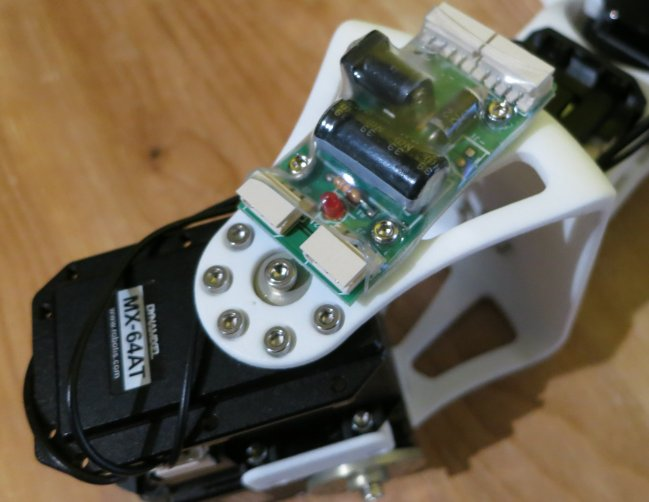
\includegraphics[width=0.8\textwidth]{screwed_SMPS}
\end{center}
\end{itemize}


Motors list:

\begin{center}

\begin{tabular}{|c|c|c|c|}
\hline 
Sub-assembly name & Motor name & Type & ID \\ 
\hline 

Double MX64 & abs\_y & MX-64AT & 31 \\ 
\hline 
Double MX64 & abs\_x & MX-64AT & 32 \\
\hline 
Spine & abs\_z & MX-28AT & 33 \\
\hline 
Double MX28 & bust\_y & MX-28AT & 34 \\
\hline 
Double MX28 & bust\_x & MX-28AT & 35 \\
\hline 
Chest & head\_z & AX-12A & 36 \\ 
\hline 
Chest & l\_shoulder\_y & MX-28AT & 41 \\
\hline 
Chest & r\_shoulder\_y & MX-28AT & 51 \\
\hline 
\end{tabular} 
\end{center}


\subsection{Arms} 
 
Documentation links:

\begin{itemize}
\item \textbf{\href{https://github.com/poppy-project/Poppy-basic-arms/blob/master/doc/subassemblies/right\_forearm\_assembly\_instructions.md}{Right}/\href{https://github.com/poppy-project/Poppy-basic-arms/blob/master/doc/subassemblies/left\_forearm\_assembly\_instructions.md}{Left} forearm} The hand design slightly changed from the videos, but the nuts and screws remain the same.
\begin{center}
  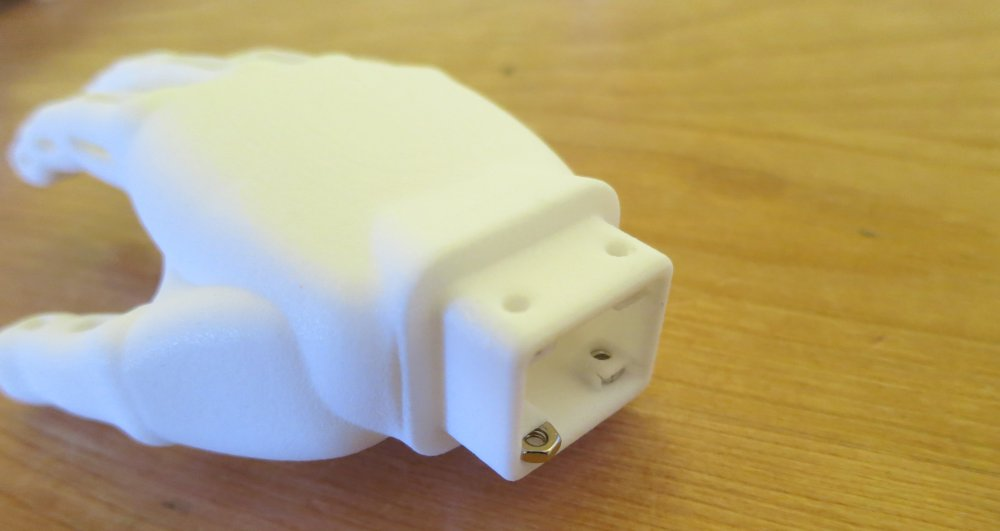
\includegraphics[width=0.8\textwidth]{hand_nut}
\end{center}
\item \textbf{\href{https://github.com/poppy-project/Poppy-basic-arms/blob/master/doc/subassemblies/right\_upper\_arm\_assembly.md}{Right}/\href{https://github.com/poppy-project/Poppy-basic-arms/blob/master/doc/subassemblies/left\_upper\_arm\_assembly.md}{Left} upper arm} Plug a 200mm cable in the unused plug before screwing the arm\_z motors (ids 43 and 53), because it will be really hard to plug once the motor is inside the structure part.
\item \textbf{\href{https://github.com/poppy-project/Poppy-basic-arms/blob/master/doc/subassemblies/right\_upper\_arm\_shoulder\_assembly.md}{Right}/\href{https://github.com/poppy-project/Poppy-basic-arms/blob/master/doc/subassemblies/left\_upper\_arm\_shoulder\_assembly.md}{Left} upper arm/shoulder}
\item \textbf{\href{https://github.com/poppy-project/Poppy-basic-arms/blob/master/doc/right\_arm\_assembly\_instructions.md}{Right}/\href{https://github.com/poppy-project/Poppy-basic-arms/blob/master/doc/left\_arm\_assembly\_instructions.md}{Left} arm assembly}
\item \textbf{\href{https://github.com/poppy-project/poppy-humanoid/blob/master/hardware/doc/Poppy\_Humanoid\_assembly\_instructions.md}{Trunk and arms assembly}} To distinguish between left and right shoulder parts, look at the three dots: the single dot should be down when the shoulder is in "zero" position (along the shoulder\_y motor).
\end{itemize}


Motors lists:

\begin{center}

\begin{tabular}{|c|c|c|c|}
\hline 
Sub-assembly name & Motor name & Type & ID \\ 
\hline 

Left upper arm/shoulder & l\_shoulder\_x & MX-28AT & 42 \\ 
\hline 
Left upper arm & l\_arm\_z & MX-28AT & 43 \\
\hline 
Left upper arm & l\_elbow\_y & MX-28AT & 44 \\
\hline 

\end{tabular} 
\end{center}

\begin{center}
\begin{tabular}{|c|c|c|c|}
\hline 
Sub-assembly name & Motor name & Type & ID \\ 
\hline 

Right upper arm/shoulder & r\_shoulder\_x & MX-28AT & 52 \\ 
\hline 
Right upper arm & r\_arm\_z & MX-28AT & 53 \\
\hline 
Right upper arm & r\_elbow\_y & MX-28AT & 54 \\
\hline 

\end{tabular} 
\end{center}


\subsection{Legs} 
 
Documentation links:

There is only a video for left leg assembly. While assembling the right leg, be sure to put your motors symetrical compared to the left leg. Also don't forget to change the motors ID from 12-15 to 22-25.

\begin{itemize}
\item \textbf{\href{https://github.com/poppy-project/Poppy-lightweight-biped-legs/blob/master/doc/subassemblies/left\_hip\_assembly\_instructions.md}{Hip}}
\item \textbf{\href{https://github.com/poppy-project/Poppy-lightweight-biped-legs/blob/master/doc/subassemblies/left\_thigh\_assembly\_instructions.md}{Tight}}
\item \textbf{\href{https://github.com/poppy-project/Poppy-lightweight-biped-legs/blob/master/doc/subassemblies/left\_shin\_assembly\_instructions.md}{Shin}}
\item \textbf{\href{https://github.com/poppy-project/Poppy-lightweight-biped-legs/blob/master/doc/subassemblies/right\_leg\_assembly\_instructions.md}{Right}/\href{https://github.com/poppy-project/Poppy-lightweight-biped-legs/blob/master/doc/subassemblies/left\_leg\_assembly\_instructions.md}{Left} leg assembly}
\item \textbf{\href{https://github.com/poppy-project/Poppy-lightweight-biped-legs/blob/master/doc/subassemblies/pelvis\_assembly\_instructions.md}{Pelvis}} The videos shows \diameter 2x5mm screws. Use the \diameter 2x5mm screws that you can find in the Bolt-nut set BNS-10.
\item \textbf{\href{https://github.com/poppy-project/poppy-humanoid/blob/master/hardware/doc/Poppy\_Humanoid\_assembly\_instructions.md}{Torso and legs assembly}}
\end{itemize}


Motors lists:

\begin{center}

\begin{tabular}{|c|c|c|c|}
\hline 
Sub-assembly name & Motor name & Type & ID \\ 
\hline 
Pelvis & l\_hip\_x & MX-28AT & 11 \\ 
\hline 
Left hip & l\_hip\_z & MX-28AT & 12 \\ 
\hline 
Left hip & l\_hip\_y & MX-64AT & 13 \\ 
\hline 
Left thigh & l\_knee\_y & MX-28AT & 14 \\ 
\hline 
Left shin & l\_ankle\_y & MX-28AT & 15\\
\hline 
\end{tabular} 
\end{center}

\begin{center}

\begin{tabular}{|c|c|c|c|}
\hline 
Sub-assembly name & Motor name & Type & ID \\ 
\hline 
Pelvis & r\_hip\_x & MX-28AT & 21 \\ 
\hline 
Right hip & r\_hip\_z & MX-28AT & 22 \\ 
\hline 
Right hip & r\_hip\_y & MX-64AT & 23 \\ 
\hline 
Right thigh & r\_knee\_y & MX-28AT & 24 \\ 
\hline 
Right shin & r\_ankle\_y & MX-28AT & 25\\
\hline 
\end{tabular} 
\end{center}


\subsection{Head} 
 
Documentation links:

Motors lists:

\begin{center}

\begin{tabular}{|c|c|c|c|}
\hline 
Sub-assembly name & Motor name & Type & ID \\ 
\hline 

Head & head\_y & AX-12A & 37 \\ 
\hline 
\end{tabular} 
\end{center}


\section{Addressing Dynamixel motors}
\label{addressing-poppys-motors}

By default, every Dynamixel servomotor has its ID set to 1. To use several servomotors in a serial way, each of them must have a unique ID.

\subsection{Installing the driver for USB2AX}

USB2AX is the device that will connect the Poppy Humanoid robot's head to the Dynamixel servomotors. It can also be used to control the servomotors directly from your computer and that's what we will do to address the motors.

On Linux, no installation is needed, but you must add yourself in the dialout group to have access to the USB port:
 \begin{verbatim}
sudo addgroup "username" dialout
\end{verbatim}

Otherwise, the driver is available \href{http://www.xevelabs.com/doku.php?id=product:usb2ax:quickstart}{here}.

Don't forget to power up your motors (using a SMPS2Dynamixel) otherwise they won't be detected !

\subsection{Installing the scanning software}

Use one of the two following softwares to access the Dynamixel servomotors regiters:

\begin{itemize}
\item \href{http://poppy-project.github.io/pypot/herborist.html}{Herborist}: tool created by the Poppy Project team. 
\item \href{http://support.robotis.com/en/software/roboplus/dynamixel_monitor/quickstart/dynamixel\_monitor\_connection.htm}{Dynamixel Wizard}: windows-only tool provided by Robotis.
\end{itemize}

Herborist comes with the Pypot library, but needs the additional library PyQt4 for graphical interface.
\begin{verbatim}
sudo pip install pypot
sudo apt-get install python-qt4
\end{verbatim}

It should then be directly accessible for a terminal:
\begin{verbatim}
sudo herborist
\end{verbatim}
 \begin{center}
  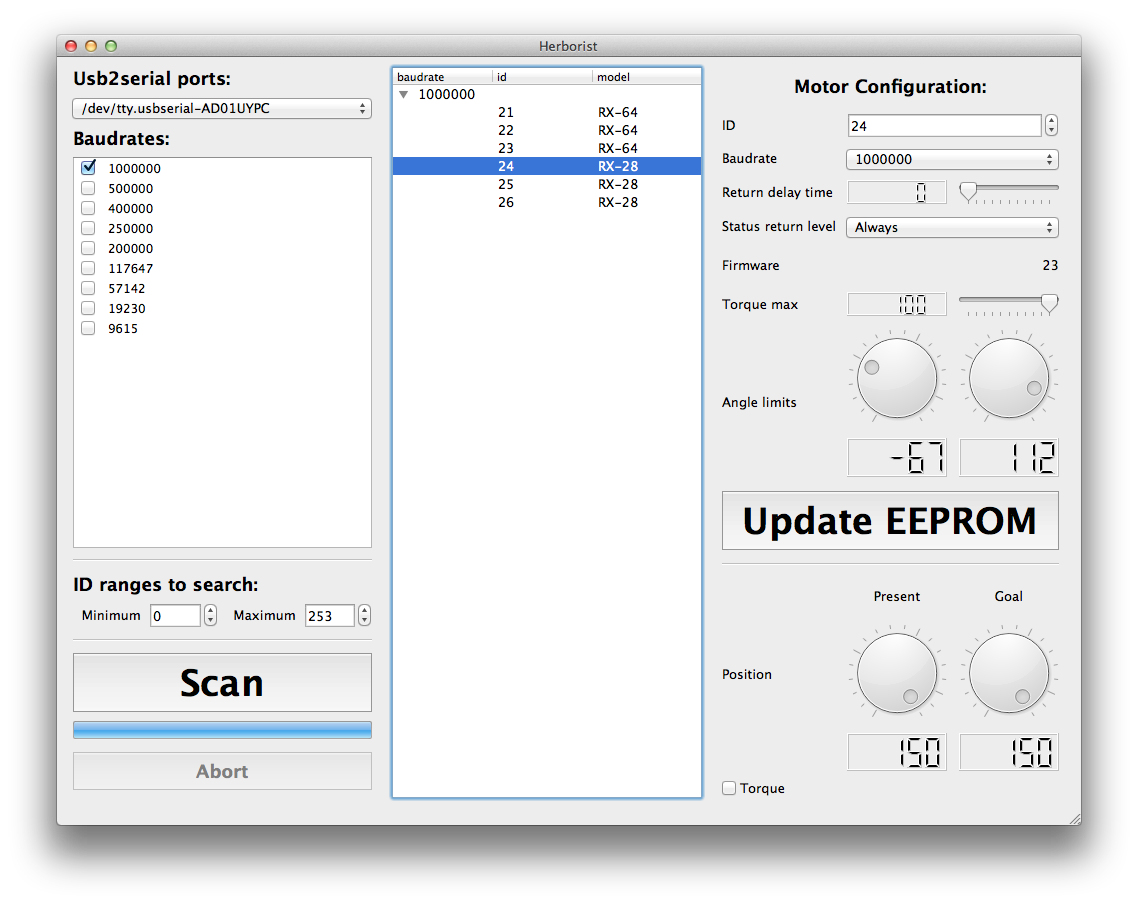
\includegraphics[width=0.8\textwidth]{herborist}
 \end{center}
 
 Connect each motor \textbf{one by one} to the USB2AX and use the 'scan' button in Herborist or Dynamixel Wizard to detect it. If it's a new motor, it should have ID 1 and baudrate 57142bps, appart AX-12A servos who already have a 1000000 baudrate.

You have to set:
\begin{itemize}
\item ID corresponding to the naming convention
\item Baudrate to 1 000 000bps
\item Return delay time to 0 ms instead of 0.5 ms
\end{itemize}

In Herborist, don't forget to click on the 'Update EEPROM' button so the changes are taken in account.


\subsection{Naming conventions}

If you want your PoppyHumanoid object to correspond to your robot without having to modify the configuration file, you should stick to the Poppy Humanoid robot naming and addressing convention. This will ensure that, in your code, when you use a motor's name, you will really send orders to the corresponding physical motor.
\begin{center}
  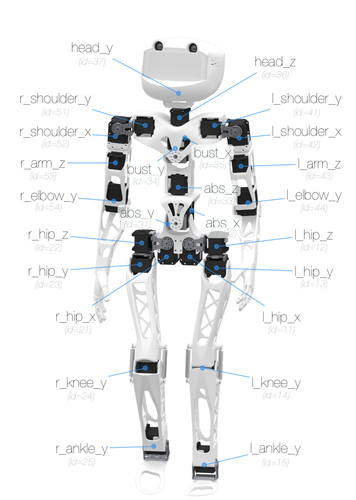
\includegraphics[width=0.7\textwidth]{motor_naming_convention}
 \end{center}
 
 
\section{Useful links}
\label{documentation-links}


\hspace{-7mm}\begin{tabular}{lr}

 \textbf{Assembly instructions:} & \href{https://github.com/poppy-project/poppy-humanoid/blob/master/hardware/doc/Poppy_Humanoid_assembly_instructions.md}{https://github.com/poppy-project/poppy-humanoid/blob/master/} \\ 

 & \href{https://github.com/poppy-project/poppy-humanoid/blob/master/hardware/doc/Poppy_Humanoid_assembly_instructions.md}{hardware/doc/Poppy\_Humanoid\_assembly\_instructions.md} \\  

 & \\

Poppy project website: & \url{https://www.poppy-project.org/} \\ 

Poppy project forum: & \url{https://forum.poppy-project.org/} \\ 

   & \\
 
Bill of Material: & \href{https://github.com/poppy-project/Poppy-lightweight-biped-legs/blob/master/doc/BOM.md}{https://github.com/poppy-project/Poppy-lightweight-biped-legs/} \\ 

 & \href{https://github.com/poppy-project/Poppy-lightweight-biped-legs/blob/master/doc/BOM.md}{/blob/master/doc/BOM.md} \\ 
 
 & \\


 
 herborist documentation & \url{http://poppy-project.github.io/pypot/herborist.html}\\
 
    & \\
   
    Dynamixel wizard doc. & \href{http://support.robotis.com/en/software/roboplus/dynamixel_monitor/quickstart/dynamixel\_monitor\_connection.htm}
{http://support.robotis.com/en/software/roboplus/}\\

     & \href{http://support.robotis.com/en/software/roboplus/dynamixel_monitor/quickstart/dynamixel\_monitor\_connection.htm}
{dynamixel\_monitor/quickstart/dynamixel\_monitor\_connection.htm}\\

   & \\

STL files: & \href{https://github.com/poppy-project/poppy-humanoid/releases/download/Official_1.0_Hardware_release/STL_3D_printed_parts.zip}{https://github.com/poppy-project/poppy-humanoid/releases/} \\ 
 & \href{https://github.com/poppy-project/poppy-humanoid/releases/download/Official_1.0_Hardware_release/STL_3D_printed_parts.zip}{download/Official\_1.0\_Hardware\_release/STL\_3D\_printed\_parts.zip}
\\

 & \\
 
\end{tabular} 



\end{document}